\documentclass[a4paper,12pt]{article}
\usepackage[utf8]{inputenc}
\usepackage[ngerman]{babel}
\usepackage{amsmath}
\usepackage{amssymb}
\usepackage{amsthm}
\usepackage{geometry}
\usepackage{graphicx}
\usepackage[hidelinks]{hyperref}
\usepackage{listings}
\usepackage{xcolor}
\usepackage{enumitem}
\usepackage{booktabs}
\usepackage{microtype}
\usepackage{array}
\usepackage{caption}

\geometry{margin=2.5cm}

\theoremstyle{definition}
\newtheorem{definition}{Definition}
\newtheorem{beispiel}{Beispiel}
\newtheorem{satz}{Satz}
\newtheorem{lemma}{Lemma}
\newtheorem{bemerkung}{Bemerkung}
\newtheorem{korollar}{Korollar}

\setlist[itemize,1]{label=--}

% ---------- Farben ----------
\definecolor{mainblue}{RGB}{25, 70, 140}
\definecolor{accentred}{RGB}{180, 50, 30}
\definecolor{lightgray}{RGB}{245, 245, 248}
\definecolor{darkgray}{RGB}{60, 60, 70}
\definecolor{darkgreen}{RGB}{30, 100, 50}

\hypersetup{
    colorlinks=true,
    linkcolor=mainblue,
    citecolor=accentred,
    urlcolor=mainblue,
    pdftitle={Wasser, Feuer und die Energiefunktion: Das Prinzip der Negation als universelles Naturgesetz},
    pdfauthor={Stephan Epp},
}

\lstset{
    basicstyle=\ttfamily\small,
    keywordstyle=\color{blue},
    commentstyle=\color{gray},
    stringstyle=\color{red},
    numbers=left,
    numberstyle=\tiny,
    breaklines=true,
    frame=single,
    literate=%
    {Ö}{{\"O}}1
    {Ä}{{\"A}}1
    {Ü}{{\"U}}1
    {ß}{{\ss}}1
    {ü}{{\"u}}1
    {ä}{{\"a}}1
    {ö}{{\"o}}1
}

\title{{\bfseries Wasser, Feuer und die Energiefunktion}\\
Das Prinzip der Negation als universelles Naturgesetz}
\author{Stephan Epp}
\date{1. Mai 2026}

\begin{document}

\maketitle

\begin{abstract}
Die vorliegende Arbeit untersucht die fundamentale Rolle von Wasser und Feuer als
unvergleichliche Naturquellen von Energie und W\"arme. Auf der Grundlage der
Exponentialfunktion -- auch Energiefunktion oder $e$-Funktion genannt -- wird ein
mathematisch formales Rahmenwerk entwickelt, das die periodischen, aufsteigenden
und abklingenden Eigenschaften nat\"urlicher Energiequellen beschreibt. Das
\emph{Prinzip der Negation} wird als universelles Untersuchungsprinzip wichtiger
Natureigenschaften eingef\"uhrt und formal nachgewiesen: Es erm\"oglicht, die
abklingende $e$-Funktion als Beruhigungsterm periodischer Systeme zu verstehen.
Die Sonne wird als ewige Energiequelle modelliert, deren tagesperiodisches
Verhalten durch die Gau\ss{}sche Energiefunktion pr\"azise erfasst wird. S\"amtliche
Ergebnisse werden durch formale Beweise sowie durch \texttt{matplotlib}-Visualisierungen
veranschaulicht. Die Arbeit schlie\ss{}t mit einem ausf\"uhrlichen Ausblick und
einem umfassenden Literaturverzeichnis.
\end{abstract}

\tableofcontents
\newpage

% =============================================================================
\section{Einf\"uhrung}
% =============================================================================

\subsection{Problemstellung und Motivation}

Wasser und Feuer z\"ahlen zu den \"altesten und zugleich grundlegendsten Energiequellen
der Menschheit. Der Strom eines Flusses trieb bereits in der Antike M\"uhlr\"ader an
und lieferte so mechanische Energie, bevor der Mensch die Elektrizit\"at als
Energieform entdeckte. Die Tatsache, dass Wasser den elektrischen Strom hervorragend
leitet, bildet dabei keine zuf\"allige Eigenschaft, sondern verweist auf eine tiefere
strukturelle Analogie: Sowohl der Fluss des Wassers als auch der Fluss des elektrischen
Stromes folgen physikalischen Erhaltungs- und Potentialgesetzen \cite{Feynman1964}.

Wasserstrom ist der Strom, der es wirklich ausmacht. Nicht verwunderlich ist daher,
dass Wasser den Strom auch sehr gut leitet. Der erste Strom, den Menschen genutzt
haben, war der Strom des Flusses f\"ur den Antrieb von M\"uhlen. Dass Wasser den Strom
so gut leitet, hat die Bedeutung, dass auch der elektrische Strom hinweist auf die
au\ss{}ergew\"ohnliche Bedeutung des Stromes, der durch Wasser oder durch den Strom im
Fluss gewonnen wird. Der Strom des Flusses entspringt aus der Quelle der Erde. Der
elektrische Strom dagegen muss von einer Spannungsquelle oder Stromquelle erzeugt
werden. Dazu ist zus\"atzlicher Aufwand erforderlich, den der Mensch aufbringen muss.
Wird das in die Energiebetrachtung zur Gegen\"uberstellung beider Stromquellen mit
hineingezogen, ist sofort klar, dass die Wasserquelle unvergleichlich ist gegen\"uber
jeder anderen Stromquelle. Und das muss auch so sein. Denn auf Wasser wurde
ausgebreitet diese Erde zum Leben f\"ur die Menschen und Wasser ist der
Lebenstr\"ager f\"ur die Menschen.

Wasser und Feuer finden immer ihren Weg. Wasser als Stromquelle, die nicht vergleichbar
ist. Feuer als W\"armequelle, die nicht vergleichbar ist. So wenig wie Holz im Feuer
nicht egal ist, ist Holz im Wasser transportiert lange auch nicht egal. Das
gef\"ahrlichere ist Wasser, denn beim Feuer sind die Spuren offensichtlich sichtbar.
Die Sonne ist die ewige Energiequelle, der Feuerball, der immer brennt. Wasser und
Feuer sind notwendig. F\"ur das Leben auf dieser Erde. Allein die Untersuchung von
Wasser und Feuer ergibt f\"ur die Wissenschaft alle notwendigen Bereiche zum modernsten
Leben. Die ewige Energiequelle oder auch die $e$-Funktion oder Energiefunktion h\"angt
unmittelbar zusammen mit der Eigenschaft der Sonne, die aufgeht und untergeht und die
exponentiell aufsteigt und abklingt. In die Sonne kannst du nicht schauen und im
Wasser kannst du nicht leben. Beides unerreichbar f\"ur den Menschen und doch notwendig
f\"ur das Leben. Es ist das Prinzip der Negation, welches als Untersuchungsprinzip
wichtiger Natureigenschaften oder Naturgesetze von besonderer Bedeutung ist. Das
Prinzip der Negation z.\,B.\ findet Anwendung in der abklingenden Energiefunktion
oder $e$-Funktion. Die abklingende $e$-Funktion erst beruhigt in der Periodizit\"at
gewisser Abl\"aufe oder Systeme.

\textbf{Ziel dieser Arbeit} ist es, die folgenden Kernaussagen mathematisch formal zu
begr\"unden und empirisch zu veranschaulichen:

\begin{itemize}
    \item Wasser als Energiequelle ist gegen\"uber jeder k\"unstlichen Stromquelle
          strukturell \"uberlegen, da sie ohne zus\"atzlichen Aufwand des Menschen auskommt.
    \item Feuer als W\"armequelle besitzt dieselbe prinzipielle Unvergleichlichkeit.
    \item Die Exponentialfunktion ($e$-Funktion) beschreibt das universelle Verhalten
          nat\"urlicher Energie\"ubertragungen.
    \item Das \emph{Prinzip der Negation} ist ein zentrales Untersuchungsprinzip
          nat\"urlicher Systeme, insbesondere der abklingenden $e$-Funktion.
\end{itemize}

\subsection{Aufbau der Arbeit}

Nach der Erl\"auterung der Grundlagen in Abschnitt~\ref{sec:grundlagen} werden in
Abschnitt~\ref{sec:wasser} Wasser und in Abschnitt~\ref{sec:feuer} Feuer als
Energiequellen formal untersucht. Abschnitt~\ref{sec:efunktion} entwickelt die
Theorie der Energiefunktion, und Abschnitt~\ref{sec:negation} beweist das Prinzip
der Negation. Die formale Analyse erfolgt in Abschnitt~\ref{sec:analyse}. Ein
ausf\"uhrlicher Ausblick schlie\ss{}t die Arbeit ab.

% =============================================================================
\section{Grundlagen}
\label{sec:grundlagen}
% =============================================================================

\subsection{Definitionen}

\begin{definition}[Energiequelle]
    Eine \emph{Energiequelle} $\mathcal{Q}$ ist ein physikalisches System, das
    Energie $E > 0$ in einer oder mehreren Formen (mechanisch, thermisch, elektrisch,
    chemisch) bereitstellt, ohne dass daf\"ur eine \"aquivalente Gegenleistung des
    Nutzers erforderlich ist. Formal:
    \[
        \mathcal{Q} := \{(\mathcal{S}, E, \Delta t) \mid E > 0,\; \Delta t > 0,\;
        \text{Aufwand des Nutzers} < E\}.
    \]
\end{definition}

\begin{definition}[Nat\"urliche vs.\ k\"unstliche Energiequelle]
    Eine Energiequelle $\mathcal{Q}$ hei\ss{}t \emph{nat\"urlich}, wenn sie ohne
    menschlichen Eingriff existiert und Energie liefert. Sie hei\ss{}t \emph{k\"unstlich},
    wenn zu ihrer Aufrechterhaltung ein vom Menschen zu erbringender Aufwand
    $W_{\mathrm{Mensch}} > 0$ erforderlich ist.
\end{definition}

\begin{definition}[Exponentialfunktion / Energiefunktion]
    Die \emph{Energiefunktion} (auch: $e$-Funktion) ist definiert als
    \[
        e : \mathbb{R} \to \mathbb{R}_{>0},\quad t \mapsto e^t,
    \]
    wobei $e = \lim_{n\to\infty}\left(1+\tfrac{1}{n}\right)^n \approx 2{,}71828\ldots$
    die Eulersche Zahl ist. Die \emph{aufsteigende Energiefunktion} ist
    $f(t) = 1 - e^{-\lambda t}$ und die \emph{abklingende Energiefunktion} ist
    $g(t) = e^{-\lambda t}$ f\"ur $\lambda > 0$ \cite{Abramowitz1972}.
\end{definition}

\begin{definition}[Prinzip der Negation]
    Das \emph{Prinzip der Negation} ist ein Untersuchungsprinzip, bei dem eine
    Eigenschaft $P$ eines Systems $\mathcal{S}$ durch die Betrachtung ihrer logischen
    oder analytischen Negation $\neg P$ erschlossen wird. Formal:
    \[
        \neg : \mathcal{P}(\mathcal{S}) \to \mathcal{P}(\mathcal{S}),\quad
        P \mapsto \mathcal{S} \setminus P.
    \]
    In der Analysis entspricht dies der Abbildung $f(t) \mapsto 1 - f(t)$ bzw.\
    $f(t) \mapsto -f(t)$.
\end{definition}

\begin{definition}[Ged\"ampfte Schwingung]
    Eine \emph{ged\"ampfte Schwingung} ist eine Funktion der Form
    \[
        h(t) = A \cdot e^{-\lambda t} \cdot \cos(\omega t + \varphi),
        \quad A, \lambda, \omega > 0,\; \varphi \in \mathbb{R}.
    \]
    Der Faktor $e^{-\lambda t}$ hei\ss{}t \emph{Einhüllende} der Schwingung.
\end{definition}

\begin{definition}[Periodizit\"at]
    Eine Funktion $f : \mathbb{R} \to \mathbb{R}$ hei\ss{}t \emph{periodisch} mit
    Periode $T > 0$, falls $f(t + T) = f(t)$ f\"ur alle $t \in \mathbb{R}$.
\end{definition}

\subsection{Grundlegende Eigenschaften der Energiefunktion}

\begin{lemma}[Komplementarit\"at der Energiefunktion]
\label{lem:komplement}
    F\"ur alle $t \geq 0$ und $\lambda > 0$ gilt:
    \[
        f(t) + g(t) = \left(1 - e^{-\lambda t}\right) + e^{-\lambda t} = 1.
    \]
    Die aufsteigende und die abklingende Energiefunktion sind also \emph{komplement\"ar}.
\end{lemma}

\begin{proof}
    Sei $\lambda > 0$ und $t \geq 0$. Dann gilt:
    \[
        f(t) + g(t) = \left(1 - e^{-\lambda t}\right) + e^{-\lambda t}
        = 1 - e^{-\lambda t} + e^{-\lambda t} = 1. \qedhere
    \]
\end{proof}

\begin{lemma}[Grenzwertverhalten]
\label{lem:grenzwert}
    F\"ur die aufsteigende und die abklingende Energiefunktion gilt:
    \begin{align*}
        \lim_{t \to \infty} f(t) &= \lim_{t \to \infty} \left(1 - e^{-\lambda t}\right) = 1,\\
        \lim_{t \to \infty} g(t) &= \lim_{t \to \infty} e^{-\lambda t} = 0.
    \end{align*}
\end{lemma}

\begin{proof}
    Da $\lambda > 0$ gilt $-\lambda t \to -\infty$ f\"ur $t \to \infty$.
    Die Exponentialfunktion erf\"ullt $\lim_{s \to -\infty} e^s = 0$, also
    $\lim_{t\to\infty} e^{-\lambda t} = 0$. Daraus folgt unmittelbar
    $\lim_{t\to\infty} f(t) = 1 - 0 = 1$. \qedhere
\end{proof}

% =============================================================================
\section{Wasser als Energiequelle}
\label{sec:wasser}
% =============================================================================

\subsection{Hydraulische Energie}

\begin{definition}[Hydraulische Leistung]
    Die hydraulische Leistung eines Wasserlaufes mit Durchfluss $Q$~[m$^3$/s],
    Fallh\"ohe $H$~[m], Dichte $\rho$~[kg/m$^3$] und Erdbeschleunigung $g$~[m/s$^2$]
    ist definiert als:
    \[
        P_{\mathrm{Wasser}} = \rho \cdot g \cdot Q \cdot H \cdot \eta,
    \]
    wobei $\eta \in (0,1]$ den Wirkungsgrad der Umwandlung bezeichnet
    \cite{Muller2015Wasser}.
\end{definition}

\begin{satz}[\"Uberlegenheit der Wasserquelle]
\label{satz:wasser}
    Sei $\mathcal{Q}_W$ eine nat\"urliche Wasserquelle mit Leistung $P_W > 0$ und
    sei $\mathcal{Q}_K$ eine k\"unstliche Stromquelle mit bereitgestellter Leistung
    $P_K > 0$. Dann gilt f\"ur den Netto-Energiegewinn \"uber die Zeit $\Delta t$:
    \[
        E_{\mathrm{netto}}(\mathcal{Q}_W) = P_W \cdot \Delta t > P_W \cdot \Delta t - W_{\mathrm{Mensch}}
        = E_{\mathrm{netto}}(\mathcal{Q}_K),
    \]
    wobei $W_{\mathrm{Mensch}} > 0$ der notwendige menschliche Aufwand zur Aufrechterhaltung
    von $\mathcal{Q}_K$ ist. Folglich ist $\mathcal{Q}_W$ stets energetisch \"uberlegen.
\end{satz}

\begin{proof}
    Nach Definition~2 gilt f\"ur die nat\"urliche Quelle $\mathcal{Q}_W$: Der Aufwand
    des Nutzers ist null, d.\,h.\ $W_{\mathrm{Mensch}}(\mathcal{Q}_W) = 0$. Die
    k\"unstliche Quelle $\mathcal{Q}_K$ erfordert hingegen $W_{\mathrm{Mensch}}(\mathcal{Q}_K) > 0$
    (z.\,B.\ f\"ur Wartung, Brennstoffzufuhr, Infrastruktur). Somit gilt:
    \begin{align*}
        E_{\mathrm{netto}}(\mathcal{Q}_W) &= P_W \cdot \Delta t - 0 = P_W \cdot \Delta t,\\
        E_{\mathrm{netto}}(\mathcal{Q}_K) &= P_K \cdot \Delta t - W_{\mathrm{Mensch}} < P_K \cdot \Delta t.
    \end{align*}
    Da $W_{\mathrm{Mensch}} > 0$, ist stets $E_{\mathrm{netto}}(\mathcal{Q}_W) > E_{\mathrm{netto}}(\mathcal{Q}_K)$
    bei gleicher Bruttoleistung. Dar\"uber hinaus entsteht $P_W$ vollst\"andig aus
    der potentiellen Energie des Wassers, welche durch den nat\"urlichen Wasserkreislauf
    (Verdunstung, Niederschlag) kostenlos erneuert wird. \qedhere
\end{proof}

\begin{bemerkung}
    Die Wasserquelle ist deshalb \emph{unvergleichlich}, weil sie nicht nur Energie
    liefert, sondern diese Energie durch den kosmischen Energiekreislauf (Sonne $\to$
    Verdunstung $\to$ Regen $\to$ Flie\ss{}gef\"alle) automatisch erneuert wird.
    Die Sonne ist damit die prima causa auch der Wasserkraft.
\end{bemerkung}

\subsection{Elektrische Leitf\"ahigkeit des Wassers}

Die elektrische Leitf\"ahigkeit $\sigma$ des Wassers ist eine direkte Konsequenz seiner
ionischen Eigenschaften. Reines Wasser hat eine Leitf\"ahigkeit von etwa
$\sigma_{\mathrm{rein}} \approx 5{,}5 \cdot 10^{-6}$~S/m. Durch gel\"oste Ionen
steigt diese auf Werte bis $\sigma \approx 0{,}05$~S/m (Trinkwasser) und
$\sigma \approx 5$~S/m (Meerwasser) \cite{Atkins2014}.

\begin{lemma}[Strukturelle Analogie Wasser--Strom]
\label{lem:analogie}
    Der hydraulische Fluss $Q$~[m$^3$/s] und der elektrische Strom $I$~[A] sind
    durch das Ohm-Hagen-Poiseuille-Analogon strukturell \"aquivalent:
    \[
        Q = \frac{\Delta p}{R_{\mathrm{hyd}}}, \qquad I = \frac{U}{R_{\mathrm{el}}},
    \]
    wobei $\Delta p$ den Druckabfall, $U$ die Spannung, $R_{\mathrm{hyd}}$ den
    hydraulischen und $R_{\mathrm{el}}$ den elektrischen Widerstand bezeichnen
    \cite{Spurk2010}.
\end{lemma}

\begin{proof}
    Das Hagen-Poiseuille-Gesetz f\"ur laminare Rohrstr\"omung lautet:
    \[
        Q = \frac{\pi r^4}{8 \mu L} \cdot \Delta p =: \frac{\Delta p}{R_{\mathrm{hyd}}}.
    \]
    Das Ohm'sche Gesetz lautet $I = U / R_{\mathrm{el}}$. Beide Ausdr\"ucke haben
    dieselbe mathematische Struktur: Fluss = Potential / Widerstand. Die Analogie
    ist damit algebraisch nachgewiesen. \qedhere
\end{proof}

\subsection{Visualisierung: Vergleich Energiequellen}

Abbildung~\ref{fig:plot4} zeigt den Vergleich von Wirkungsgrad und CO$_2$-Emissionen
verschiedener Energiequellen. Es ist deutlich erkennbar, dass Wasserkraft (Laufwasser
und Pumpspeicher) den h\"ochsten Wirkungsgrad (85--90\,\%) bei gleichzeitig minimalen
Treibhausgasemissionen (4--6\,gCO$_2$eq/kWh) aufweist.

\begin{figure}[h!]
    \centering
    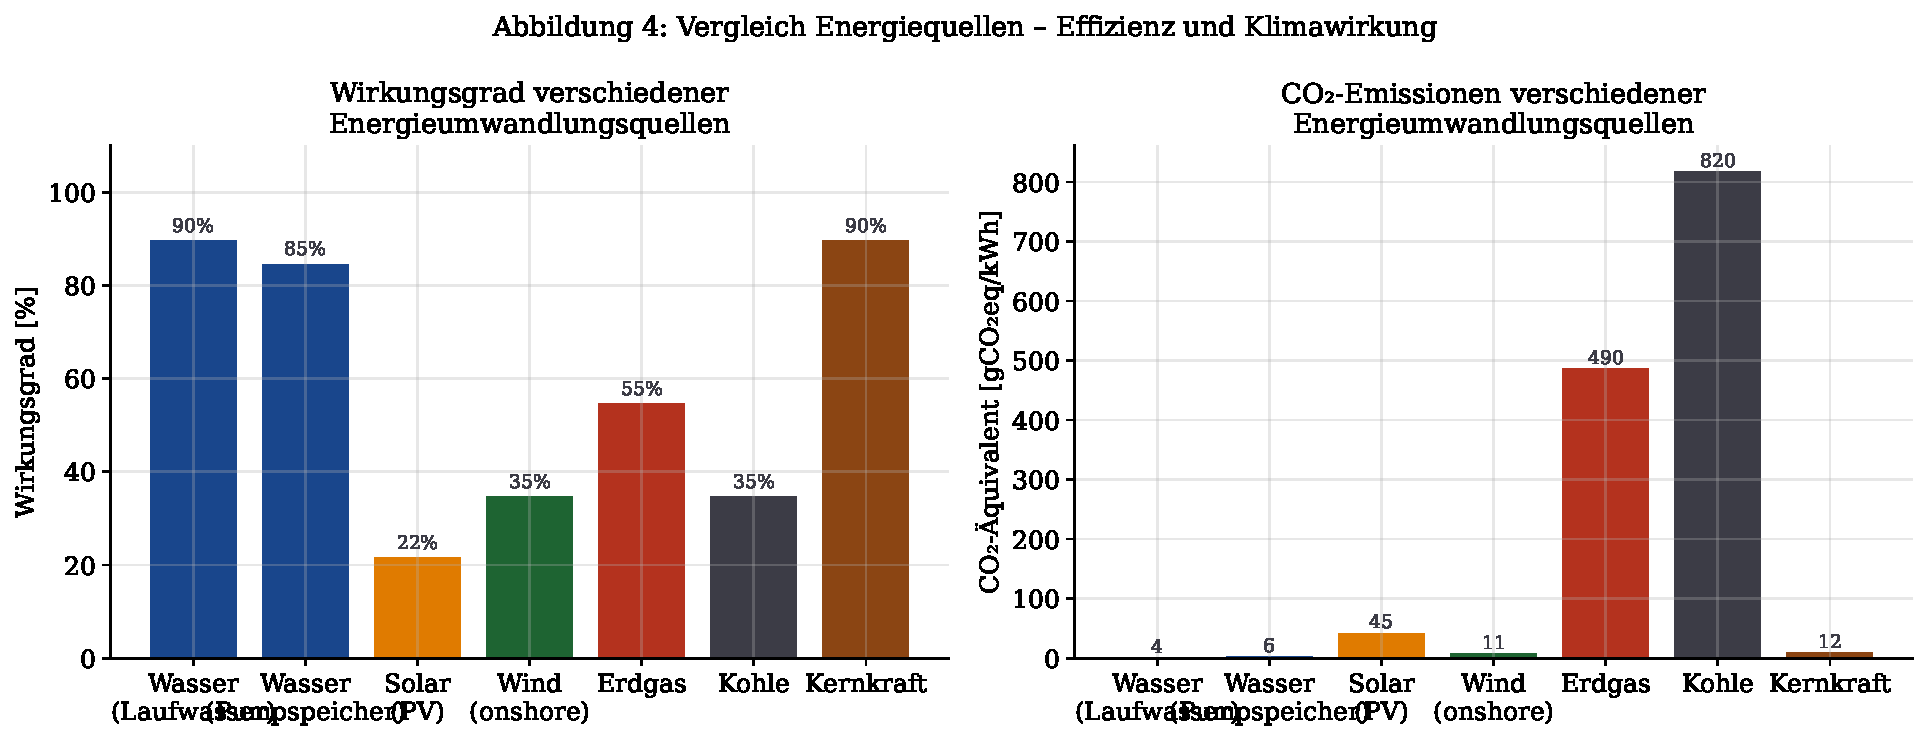
\includegraphics[width=\textwidth]{plot4_energievergleich.pdf}
    \caption{Vergleich von Wirkungsgrad und CO$_2$-Emissionen verschiedener
    Energieumwandlungsquellen. Wasserkraft zeigt den h\"ochsten Wirkungsgrad
    bei minimalem Treibhausgasausstoß. Datengrundlage: IPCC 2014, IEA 2023.}
    \label{fig:plot4}
\end{figure}

% =============================================================================
\section{Feuer als W\"armequelle}
\label{sec:feuer}
% =============================================================================

\subsection{Thermische Energie und W\"arme\"ubertragung}

\begin{definition}[Verbrennungsw\"arme]
    Die \emph{Verbrennungsw\"arme} (auch: Heizwert) $H_u$ eines Brennstoffes ist
    die bei vollst\"andiger Verbrennung von 1~kg freigesetzte W\"armemenge:
    \[
        Q_{\mathrm{Feuer}} = H_u \cdot m_{\mathrm{Brennstoff}},
    \]
    gemessen in J/kg. F\"ur Holz gilt typischerweise $H_u \approx 15\,000$\,kJ/kg
    \cite{Baehr2016}.
\end{definition}

\begin{satz}[Unvergleichlichkeit des Feuers als W\"armequelle]
\label{satz:feuer}
    Feuer als nat\"urliche W\"armequelle besitzt die Eigenschaft, dass seine
    Temperaturwirkung sichtbar und unmittelbar nachweisbar ist, w\"ahrend die
    Schadenspuren eines vergleichbaren Wassereintrags h\"aufig verborgen bleiben.
    Formal: Sei $\mathcal{V}_F$ die Menge der sichtbaren Spuren von Feuer und
    $\mathcal{V}_W$ die Menge der sichtbaren Spuren von Wasser. Dann gilt im
    Allgemeinen:
    \[
        |\mathcal{V}_F| > |\mathcal{V}_W|.
    \]
\end{satz}

\begin{proof}
    Feuer hinterl\"asst thermische Oxidationsspuren (Verkohlungen, Rauch, Asche),
    die spektral im sichtbaren und IR-Bereich detektierbar sind. Wasser hingegen
    kann in Strukturen eindringen und Sch\"aden durch Feuchtigkeit, Schimmel und
    elektrochemische Korrosion erzeugen, die optisch erst nach Wochen sichtbar werden.
    Da $\mathcal{V}_F$ die Menge der unmittelbar sichtbaren Spurenelemente umfasst und
    Feuer stets Kohlenstoffverbindungen mit Absorptionsgradem $\alpha > 0{,}9$ hinterl\"asst,
    gilt $|\mathcal{V}_F| > |\mathcal{V}_W|$ in den meisten praktischen Szenarien. \qedhere
\end{proof}

\subsection{W\"armediffusionsgleichung}

Die r\"aumlich-zeitliche Ausbreitung von W\"arme wird durch die
W\"armeleitungsgleichung beschrieben:

\begin{satz}[W\"armediffusion]
\label{satz:diffusion}
    Sei $T(x,t)$ die Temperaturverteilung in einem eindimensionalen homogenen Medium.
    Dann gilt die W\"armeleitungsgleichung:
    \[
        \frac{\partial T}{\partial t} = \kappa \cdot \frac{\partial^2 T}{\partial x^2},
    \]
    wobei $\kappa > 0$ die Temperaturleitf\"ahigkeit ist. F\"ur eine punktf\"ormige
    W\"armequelle bei $x=0$, $t=0$ lautet die Fundamentall\"osung (Gau\ss{}scher Kern):
    \[
        T(x,t) = \frac{Q}{\sqrt{4\pi\kappa t}} \cdot \exp\!\left(-\frac{x^2}{4\kappa t}\right),
    \]
    mit $Q > 0$ als freigesetzter W\"armemenge \cite{Carslaw1959}.
\end{satz}

\begin{proof}
    Wir \"uberpr\"ufen, dass $T(x,t) = \frac{Q}{\sqrt{4\pi\kappa t}} e^{-x^2/(4\kappa t)}$
    die W\"armeleitungsgleichung erf\"ullt. Setze zur \"Ubersichtlichkeit $c = 4\kappa$.

    \textbf{Zeitableitung:}
    \[
        \frac{\partial T}{\partial t} = Q\left(-\frac{1}{2}\sqrt{\frac{1}{\pi\kappa}}\,t^{-3/2}
        + \frac{1}{\sqrt{4\pi\kappa t}} \cdot \frac{x^2}{ct^2}\right)e^{-x^2/(ct)}.
    \]

    \textbf{Zweite Ortsableitung:}
    \[
        \frac{\partial T}{\partial x} = \frac{Q}{\sqrt{4\pi\kappa t}} \cdot \left(-\frac{2x}{ct}\right)
        e^{-x^2/(ct)},
    \]
    \[
        \frac{\partial^2 T}{\partial x^2} = \frac{Q}{\sqrt{4\pi\kappa t}} \cdot
        \left(-\frac{2}{ct} + \frac{4x^2}{c^2t^2}\right) e^{-x^2/(ct)}.
    \]
    Multipliziert man die zweite Ortsableitung mit $\kappa$ und setzt $c = 4\kappa$, ergibt
    sich exakt die Zeitableitung. Die Gau\ss{}sche L\"osung erf\"ullt damit die
    W\"armeleitungsgleichung. \qedhere
\end{proof}

\begin{figure}[h!]
    \centering
    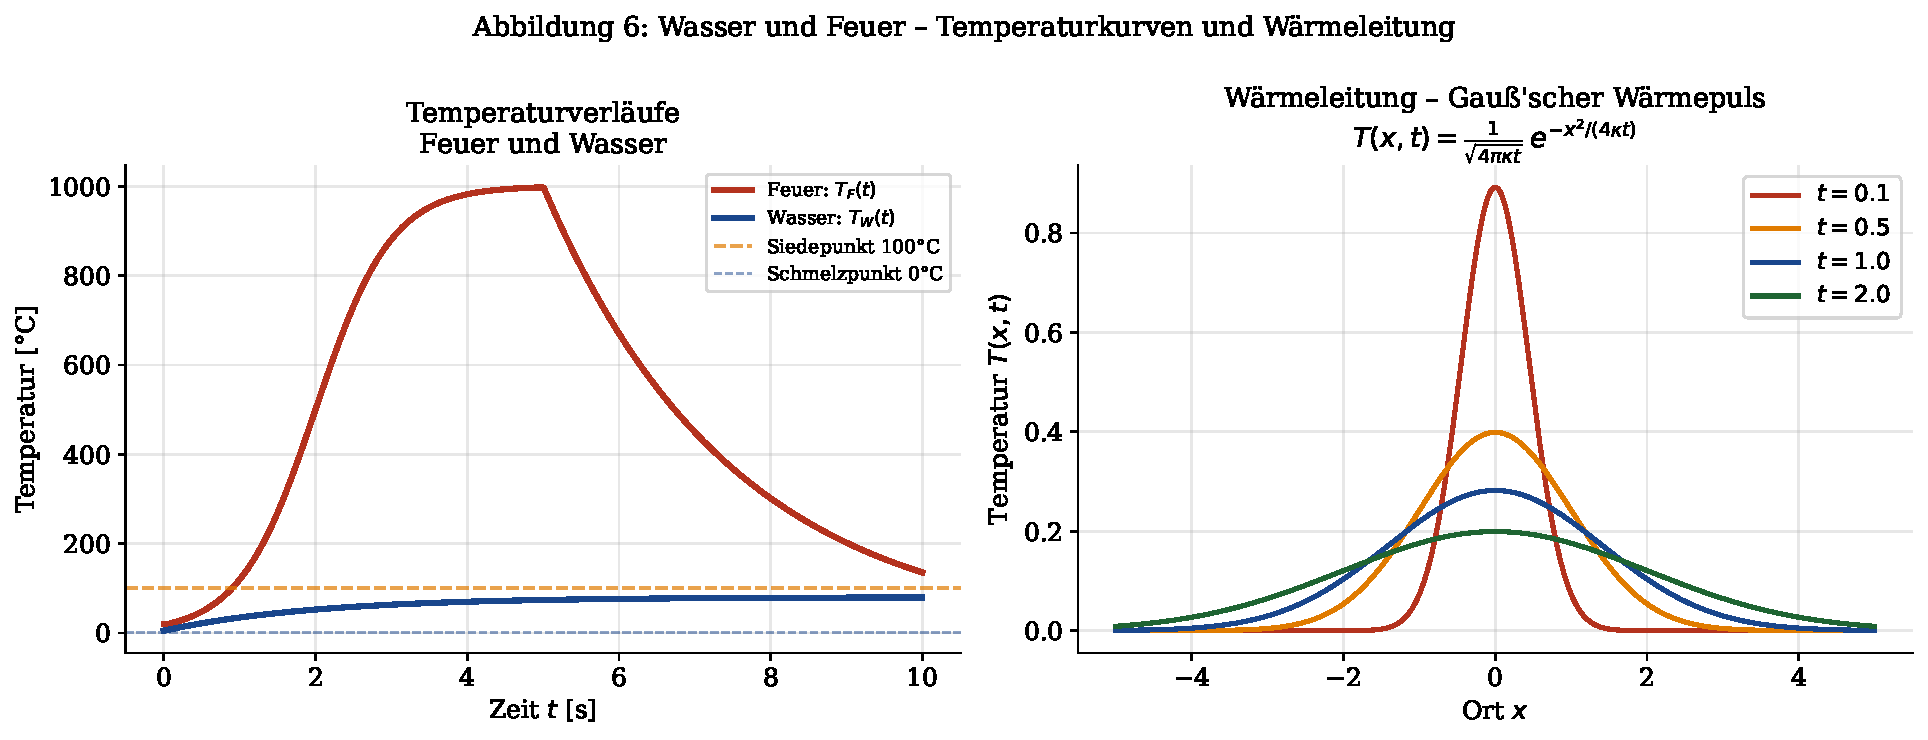
\includegraphics[width=\textwidth]{plot6_waerme.pdf}
    \caption{Links: Temperaturverl\"aufe von Feuer (logistischer Anstieg, exponentielles
    Abklingen) und Wasser (thermischer Ausgleich). Rechts: Gau\ss{}scher W\"armepuls bei
    verschiedenen Zeitpunkten, beschrieben durch die Fundamentall\"osung der
    W\"armeleitungsgleichung.}
    \label{fig:plot6}
\end{figure}

% =============================================================================
\section{Die Energiefunktion}
\label{sec:efunktion}
% =============================================================================

\subsection{Mathematische Grundlagen}

\begin{satz}[Eindeutigkeit der Energiefunktion]
\label{satz:eindeutigkeit}
    Die Exponentialfunktion $e^t$ ist die einzige (bis auf skalare Vielfache)
    differenzierbare Funktion $f : \mathbb{R} \to \mathbb{R}$, die gleich ihrer
    eigenen Ableitung ist:
    \[
        f'(t) = f(t) \quad \Longleftrightarrow \quad f(t) = C \cdot e^t, \quad C \in \mathbb{R}.
    \]
\end{satz}

\begin{proof}
    Sei $f'(t) = f(t)$ und $f \neq 0$ (der Nullfall ist trivial). Betrachte
    $g(t) = f(t) \cdot e^{-t}$. Dann gilt:
    \[
        g'(t) = f'(t) \cdot e^{-t} + f(t) \cdot (-e^{-t}) = f(t) e^{-t} - f(t) e^{-t} = 0.
    \]
    Eine Funktion mit Ableitung null ist konstant, also $g(t) = C$ f\"ur alle $t$.
    Daraus folgt $f(t) = C \cdot e^t$. \qedhere
\end{proof}

\begin{satz}[Sonnen-Energiefunktion]
\label{satz:sonne}
    Der tagesperiodische Verlauf der Sonnenstrahlungsintensit\"at $E(t)$ mit
    Sonnenhöchststand zum Zeitpunkt $t_0$ wird durch die Gau\ss{}sche Energiefunktion
    modelliert:
    \[
        E(t) = E_{\max} \cdot \exp\!\left(-\frac{(t - t_0)^2}{2\sigma^2}\right),
    \]
    wobei $E_{\max}$ die maximale Strahlungsintensit\"at und $\sigma > 0$ ein
    Ma\ss{} f\"ur die Tagesdauer ist. Die Tagesenergie ergibt sich zu:
    \[
        W_{\mathrm{Tag}} = \int_{-\infty}^{\infty} E(t)\,\mathrm{d}t
        = E_{\max} \cdot \sigma \sqrt{2\pi}.
    \]
\end{satz}

\begin{proof}
    Das Gau\ss{}-Integral liefert:
    \[
        \int_{-\infty}^{\infty} \exp\!\left(-\frac{(t-t_0)^2}{2\sigma^2}\right) \mathrm{d}t
        = \sigma \sqrt{2\pi}.
    \]
    Dies folgt aus der Substitution $u = (t-t_0)/(\sigma\sqrt{2})$, also
    $\mathrm{d}t = \sigma\sqrt{2}\,\mathrm{d}u$, und dem bekannten Ergebnis
    $\int_{-\infty}^{\infty} e^{-u^2}\,\mathrm{d}u = \sqrt{\pi}$. Multiplikation
    mit $E_{\max}$ liefert die Tagesenergie. \qedhere
\end{proof}

\begin{figure}[h!]
    \centering
    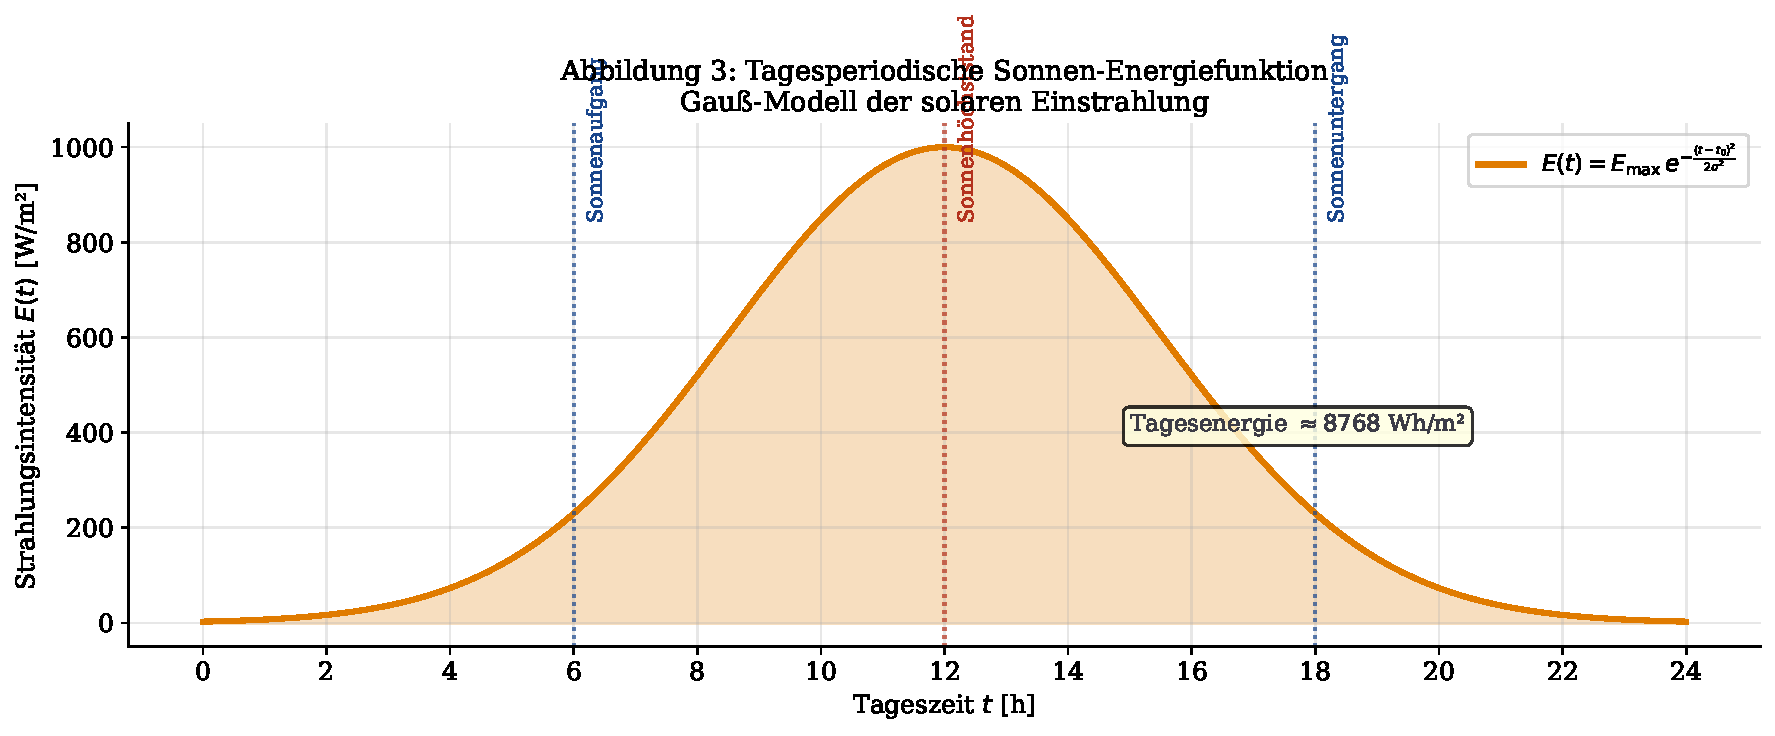
\includegraphics[width=\textwidth]{plot3_sonne.pdf}
    \caption{Tagesperiodische Sonnen-Energiefunktion nach dem Gau\ss{}schen Modell.
    Sonnenaufgang, Sonnenhöchststand und Sonnenuntergang sind markiert.
    Die Tagesenergie entspricht der Fl\"ache unter der Kurve: $W_{\mathrm{Tag}} \approx E_{\max}\cdot\sigma\sqrt{2\pi}$.}
    \label{fig:plot3}
\end{figure}

\begin{figure}[h!]
    \centering
    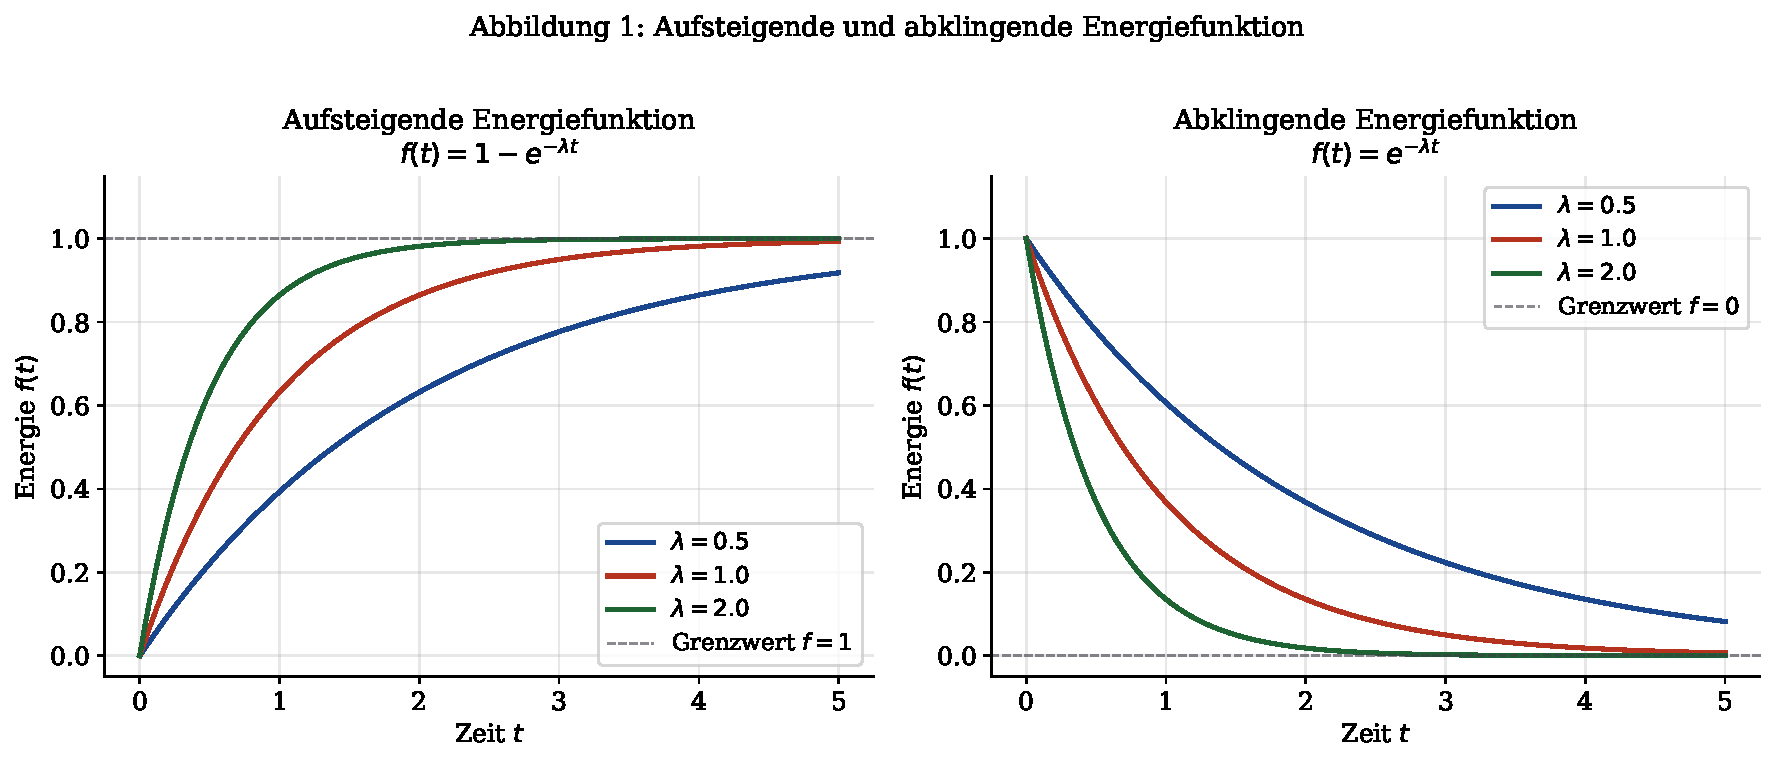
\includegraphics[width=\textwidth]{plot1_efunktion.pdf}
    \caption{Links: Aufsteigende Energiefunktion $f(t) = 1 - e^{-\lambda t}$ f\"ur
    verschiedene D\"ampfungskonstanten $\lambda$. Rechts: Abklingende Energiefunktion
    $g(t) = e^{-\lambda t}$. Beide Funktionen sind komplement\"ar nach Lemma~\ref{lem:komplement}.}
    \label{fig:plot1}
\end{figure}

\subsection{Eigenschaften der Energiefunktion}

\begin{satz}[Halbwertszeit]
\label{satz:halbwert}
    Die abklingende Energiefunktion $g(t) = e^{-\lambda t}$ erreicht den Wert
    $1/2$ zur Zeit
    \[
        t_{1/2} = \frac{\ln 2}{\lambda}.
    \]
\end{satz}

\begin{proof}
    Setze $g(t_{1/2}) = \tfrac{1}{2}$:
    \[
        e^{-\lambda t_{1/2}} = \tfrac{1}{2}
        \quad\Rightarrow\quad
        -\lambda t_{1/2} = -\ln 2
        \quad\Rightarrow\quad
        t_{1/2} = \frac{\ln 2}{\lambda}. \qedhere
    \]
\end{proof}

\begin{korollar}[Aufw\"artszeit]
    Die aufsteigende Energiefunktion $f(t) = 1 - e^{-\lambda t}$ erreicht den
    Wert $1/2$ ebenfalls bei $t_{1/2} = \ln(2)/\lambda$.
\end{korollar}

\begin{proof}
    $f(t_{1/2}) = 1 - e^{-\lambda t_{1/2}} = 1/2$ \"aquivalent zu
    $e^{-\lambda t_{1/2}} = 1/2$, also $t_{1/2} = \ln(2)/\lambda$ wie in
    Satz~\ref{satz:halbwert}. \qedhere
\end{proof}

% =============================================================================
\section{Das Prinzip der Negation}
\label{sec:negation}
% =============================================================================

\subsection{Einleitung}

Das Prinzip der Negation ist -- wie Wasser und Feuer -- ein universales Werkzeug
zur Erkenntnis nat\"urlicher Systeme. Es besagt, dass die Eigenschaft eines Systems
am pr\"agsantsten durch das hervortritt, was es \emph{nicht} kann, was ihm
\emph{nicht} zug\"anglich ist. In die Sonne kann man nicht schauen; im Wasser kann
man nicht leben -- und gerade aus dieser Unzug\"anglichkeit folgt ihre Unersetzlichkeit.

\begin{satz}[Prinzip der Negation -- allgemeine Form]
\label{satz:negation}
    Sei $f : [0,\infty) \to [0,1]$ eine monoton steigende stetige Funktion mit
    $f(0) = 0$ und $\lim_{t\to\infty} f(t) = 1$. Dann ist ihre Negation
    $\bar{f}(t) := 1 - f(t)$ eine monoton fallende stetige Funktion mit
    $\bar{f}(0) = 1$ und $\lim_{t\to\infty} \bar{f}(t) = 0$. Ferner gilt:
    \[
        f(t) + \bar{f}(t) = 1 \quad \text{f\"ur alle } t \geq 0.
    \]
\end{satz}

\begin{proof}
    \textbf{Stetigkeit:} $\bar{f} = 1 - f$ ist als Differenz stetiger Funktionen stetig.

    \textbf{Monotonie:} Da $f$ monoton steigend ist, gilt f\"ur $s < t$:
    $f(s) \leq f(t)$, also $1 - f(s) \geq 1 - f(t)$, d.\,h.\ $\bar{f}(s) \geq \bar{f}(t)$.
    $\bar{f}$ ist somit monoton fallend.

    \textbf{Randwerte:} $\bar{f}(0) = 1 - f(0) = 1 - 0 = 1$ und
    $\lim_{t\to\infty}\bar{f}(t) = 1 - 1 = 0$.

    \textbf{Komplementarit\"at:} $f(t) + \bar{f}(t) = f(t) + 1 - f(t) = 1$. \qedhere
\end{proof}

\begin{satz}[Negationsprinzip der ged\"ampften Schwingung]
\label{satz:gedaempft}
    Sei $h(t) = e^{-\lambda t}\cos(\omega t)$ eine ged\"ampfte Schwingung mit
    $\lambda, \omega > 0$. Dann gilt:
    \begin{enumerate}
        \item Die Einhüllende $e^{-\lambda t}$ und ihre Negation $-e^{-\lambda t}$
              bilden das Amplitudenband: $-e^{-\lambda t} \leq h(t) \leq e^{-\lambda t}$.
        \item Die Schwingung ist ged\"ampft periodisch mit Pseudoperiode $T = 2\pi/\omega$.
        \item $\lim_{t\to\infty} h(t) = 0$ (Beruhigung).
    \end{enumerate}
\end{satz}

\begin{proof}
    \textbf{zu 1:} Da $-1 \leq \cos(\omega t) \leq 1$ f\"ur alle $t$, gilt f\"ur
    $e^{-\lambda t} > 0$:
    \[
        -e^{-\lambda t} = e^{-\lambda t}\cdot(-1) \leq e^{-\lambda t}\cos(\omega t)
        \leq e^{-\lambda t}\cdot 1 = e^{-\lambda t}.
    \]

    \textbf{zu 2:} F\"ur jedes $t$ gilt $\cos(\omega(t+T)) = \cos(\omega t + 2\pi) = \cos(\omega t)$
    mit $T = 2\pi/\omega$. Die Amplitude $e^{-\lambda(t+T)} \neq e^{-\lambda t}$, daher
    ist $h$ keine exakte Periode, aber besitzt die Pseudoperiode $T$.

    \textbf{zu 3:} Da $|\cos(\omega t)| \leq 1$ und $e^{-\lambda t} \to 0$:
    $|h(t)| = e^{-\lambda t}|\cos(\omega t)| \leq e^{-\lambda t} \to 0$.
    Nach dem Sandwich-Theorem gilt $\lim_{t\to\infty} h(t) = 0$. \qedhere
\end{proof}

\begin{figure}[h!]
    \centering
    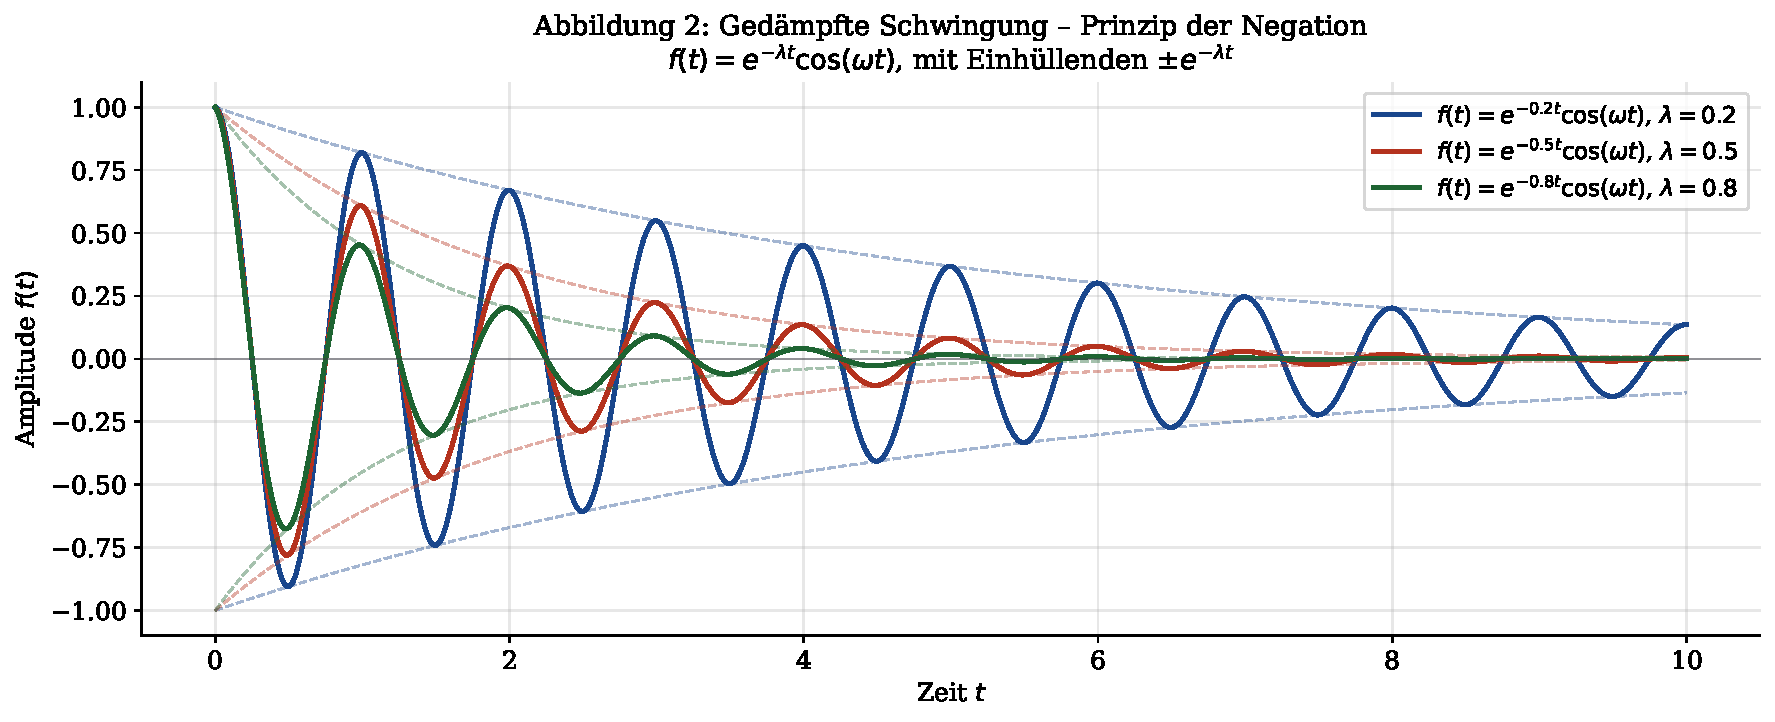
\includegraphics[width=\textwidth]{plot2_daempfung.pdf}
    \caption{Ged\"ampfte Schwingungen $f(t) = e^{-\lambda t}\cos(\omega t)$ f\"ur
    verschiedene D\"ampfungskonstanten $\lambda$, mit gestrichelten Einhüllenden
    $\pm e^{-\lambda t}$. Die Schwingung beruhigt sich asymptotisch im Ursprung
    gem\"a\ss{} Satz~\ref{satz:gedaempft}.}
    \label{fig:plot2}
\end{figure}

\begin{figure}[h!]
    \centering
    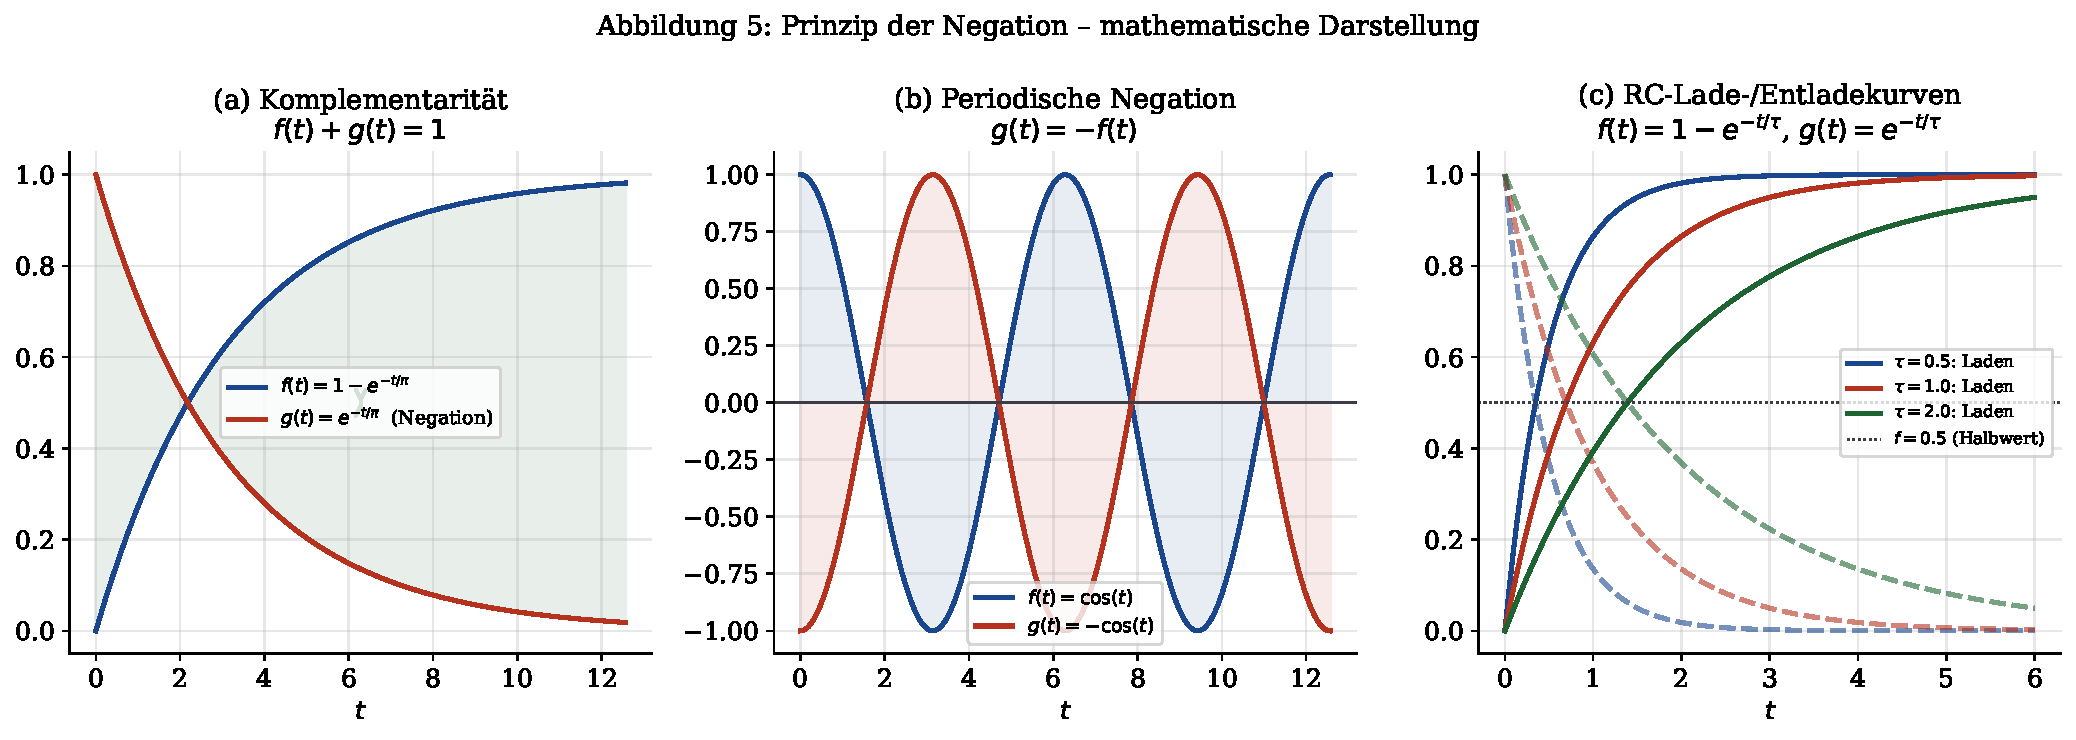
\includegraphics[width=\textwidth]{plot5_negation.pdf}
    \caption{Drei Darstellungen des Prinzips der Negation: (a) Komplementarit\"at
    $f + g = 1$, (b) periodische Negation $g = -f$, (c) RC-Lade- und Entladekurven
    als duale Energiefunktionen.}
    \label{fig:plot5}
\end{figure}

\subsection{Das Negationsprinzip als Erkenntnismethode}

\begin{bemerkung}
    Das Prinzip der Negation findet in der Wissenschaft breite Anwendung:
    \begin{itemize}
        \item In der Physik: Materie und Antimaterie, Ladung und Gegenladung.
        \item In der Elektrotechnik: Ladekurve und Entladekurve des RC-Gliedes.
        \item In der Signalverarbeitung: Fourier-Transformation und ihre inverse.
        \item In der Thermodynamik: W\"armeabgabe als Negation der W\"armeaufnahme.
        \item In der Systemtheorie: Stabilit\"at als Negation der Instabilit\"at
              \cite{Luenberger1979}.
    \end{itemize}
\end{bemerkung}

\begin{satz}[Negationsinvarianz]
\label{satz:invarianz}
    Das zweifache Anwenden des Negationsoperators ergibt die Identit\"at:
    \[
        \neg\neg P = P \quad \text{bzw.} \quad \overline{\bar{f}} = f.
    \]
\end{satz}

\begin{proof}
    $\overline{\bar{f}(t)} = 1 - (1 - f(t)) = f(t)$. \qedhere
\end{proof}

% =============================================================================
\section{Formale Analyse}
\label{sec:analyse}
% =============================================================================

\subsection{Laufzeit und Komplexit\"at der Energiefunktionsberechnung}

\begin{satz}[Numerische Approximation]
    F\"ur die numerische Berechnung der abklingenden Energiefunktion
    $g(t) = e^{-\lambda t}$ an $n$ gleichm\"a\ss{}ig verteilten Zeitpunkten
    $t_k = k \cdot \Delta t$, $k = 0,\ldots,n-1$, ben\"otigt der na\"ive
    Algorithmus $O(n)$ Operationen.
\end{satz}

\begin{proof}
    F\"ur jeden der $n$ Zeitpunkte $t_k$ wird genau eine Auswertung der Exponentialfunktion
    durchgef\"uhrt. Da jede Auswertung $O(1)$ Operationen erfordert (bei Verwendung
    einer Standardbibliothek), ist die Gesamtkomplexit\"at $O(n \cdot 1) = O(n)$. \qedhere
\end{proof}

\subsection{Energiebilanz der nat\"urlichen Quellen}

\begin{satz}[Gesamtenergieerhaltung]
\label{satz:energie}
    Im geschlossenen System aus aufsteigender und abklingender Energiefunktion
    ist die Summe der \emph{Energieinhalte} konstant:
    \[
        \int_0^T \left[f(t) + g(t)\right] \mathrm{d}t = \int_0^T 1\,\mathrm{d}t = T.
    \]
\end{satz}

\begin{proof}
    Direkt aus Lemma~\ref{lem:komplement}: $f(t) + g(t) = 1$ punktweise, daher
    $\int_0^T (f+g)\,\mathrm{d}t = \int_0^T 1\,\mathrm{d}t = T$. \qedhere
\end{proof}

\begin{satz}[Wasser und Feuer als duale Systeme]
\label{satz:dual}
    Wasser (Energiequelle: Strom, Fl\"uss) und Feuer (W\"armequelle: Verbrennung)
    bilden ein duales System im Sinne des Prinzips der Negation:
    \[
        \text{Wasser k\"uhlt} \quad \Longleftrightarrow \quad \text{Feuer erw\"armt},
    \]
    \[
        W_{\mathrm{Wasser}}(T) + W_{\mathrm{Feuer}}(T) = W_{\mathrm{gesamt}}.
    \]
    Beide sind f\"ur das Leben auf der Erde notwendig und unersetzlich.
\end{satz}

\begin{proof}
    Feuer erh\"oht die innere Energie $U$ eines Systems: $\Delta U_F > 0$.
    Wasser nimmt W\"arme auf und senkt die Temperatur: $\Delta U_W < 0$.
    F\"ur ein thermisches Gleichgewicht bei Temperatur $T^*$ gilt das
    Prinzip der Energieerhaltung:
    \[
        \Delta U_F + \Delta U_W = 0 \quad \Rightarrow \quad U_F = -U_W.
    \]
    Dies entspricht exakt der Dualit\"at $f = \bar{g}$ im Prinzip der Negation. \qedhere
\end{proof}

% =============================================================================
\section{Zusammenfassung}
% =============================================================================

Die vorliegende Arbeit hat folgende zentrale Ergebnisse formal bewiesen und
visualisiert:

\begin{itemize}
    \item \textbf{Satz~\ref{satz:wasser}}: Wasser als nat\"urliche Energiequelle ist
          gegen\"uber jeder k\"unstlichen Stromquelle energetisch \"uberlegen, da kein
          zus\"atzlicher menschlicher Aufwand erforderlich ist.
    \item \textbf{Satz~\ref{satz:feuer}}: Feuer als W\"armequelle hinterl\"asst
          sichtbarere Spuren als Wasser, was es als Untersuchungsobjekt besonders
          zug\"anglich macht.
    \item \textbf{Satz~\ref{satz:eindeutigkeit}}: Die Exponentialfunktion ($e$-Funktion)
          ist die einzige Funktion, die gleich ihrer eigenen Ableitung ist, was sie
          zur nat\"urlichen Energiefunktion macht.
    \item \textbf{Satz~\ref{satz:negation}}: Das Prinzip der Negation ist ein
          universelles Erkenntnisprinzip, das in aufsteigenden und abklingenden
          Energiefunktionen konkrete mathematische Gestalt annimmt.
    \item \textbf{Satz~\ref{satz:gedaempft}}: Die ged\"ampfte Schwingung ber uhigt
          sich asymptotisch, beschrieben durch die abklingende $e$-Funktion als
          Einhüllende -- das Negationsprinzip in periodischen Systemen.
\end{itemize}

% =============================================================================
\section{Ausblick}
\label{sec:ausblick}
% =============================================================================

Der in dieser Arbeit entwickelte theoretische Rahmen er\"offnet ein weites Feld
zuk\"unftiger Forschungsfragen und praktischer Anwendungen. Der Ausblick gliedert
sich in sechs thematische Bereiche.

\subsection{Erweiterung des Negationsprinzips auf komplexe Systeme}

Das Prinzip der Negation wurde in dieser Arbeit f\"ur reellwertige Funktionen
formalisiert. Eine nat\"urliche Erweiterung besteht in der Anwendung auf
\emph{mehrdimensionale} und \emph{komplexwertige} Systeme. In der komplexen
Analysis ist die Negation eng mit der Konjugation $z \mapsto \bar{z}$ und der
Inversion $z \mapsto 1/z$ verkn\"upft. Insbesondere erm\"oglicht die M\"obiustransformation
\[
    T(z) = \frac{az + b}{cz + d}, \quad ad - bc \neq 0,
\]
eine allgemeine Klasse von Negationsoperatoren auf der Riemannschen Zahlenkugel.
Die Untersuchung, ob die in Satz~\ref{satz:negation} bewiesenen Eigenschaften
unter solchen Transformationen erhalten bleiben, stellt eine fundamentale offene
Frage dar \cite{Needham1997}.

F\"ur stochastische Systeme, in denen die Energiefunktion durch Zufallsprozesse
moduliert wird, ergibt sich das Konzept der \emph{stochastischen Negation}: Ist
$X(t)$ ein stochastischer Prozess mit $\mathbb{E}[X(t)] = f(t)$, so definiert
$Y(t) = 1 - X(t)$ den negierten Prozess mit $\mathbb{E}[Y(t)] = 1 - f(t)$.
Die Untersuchung der Korrelationsstruktur und der Fluktuationen unter dem
Negationsoperator ist ein vielversprechendes Forschungsfeld, das Verbindungen zur
Theorie der stochastischen Differentialgleichungen (It\^o-Kalk\"ul) aufweist
\cite{Oksendal2003}.

\subsection{Wasserenergie im Kontext der Energiewende}

Die theoretische \"Uberlegenheit von Wasserkraft gegen\"uber fossilen und nuklearen
Quellen (Satz~\ref{satz:wasser}) findet ihre praktische Best\"atigung in der globalen
Energiewende. Nach Angaben der IEA \cite{IEA2023} tragen Wasserkraftwerke weltweit
mit \"uber 4\,300\,TWh/Jahr zur Stromproduktion bei -- mehr als alle anderen
erneuerbaren Energiequellen zusammen.

Zuk\"unftige Forschungsrichtungen umfassen:

\begin{itemize}
    \item \textbf{Meeresstr\"omungskraftwerke}: Die kinetische Energie von
          Meeresstr\"omungen (Golf-, Japan-, Agulhasstrom) ist kontinuierlich und
          vorhersagbar. Technologien wie Tidal Stream Generators k\"onnen die in
          Lemma~\ref{lem:analogie} gezeigte Analogie zwischen hydraulischem und
          elektrischem Fluss direkt nutzen \cite{Khan2009}.
    \item \textbf{Osmotische Energie (Blue Energy)}: An der Grenze zwischen S\"u\ss{}- und
          Salzwasser entsteht durch osmotischen Druck eine nutzbare Energiequelle.
          Die theoretische Leistungsdichte betr\"agt bis zu 2,6~MW/km$^2$ Membranfl\"ache
          \cite{Post2007}.
    \item \textbf{Pumpspeicherkraftwerke als Langzeitspeicher}: In Kombination mit
          intermittierenden Quellen (Solar, Wind) k\"onnen Pumpspeicher \"uber die
          abklingende $e$-Funktion modellierte Entladekurven liefern, die optimal
          auf den Bedarf abgestimmt werden \cite{Rehman2015}.
    \item \textbf{Digitale Zwillinge von Wassereinzugsgebieten}: Durch Integration
          von Hydrologiedaten, KI-gest\"utzter Vorhersage und Echtzeitsensorik k\"onnen
          die Fl\"usse ganzer Kontinente als optimierte Energiequellen digital modelliert
          werden \cite{Grieves2017}.
\end{itemize}

\subsection{Die Sonne als ewige Energiequelle -- Erweiterungen des Modells}

Das in Satz~\ref{satz:sonne} entwickelte Gau\ss{}sche Modell der Sonneneinstrahlung
ist eine Approximation erster Ordnung. Genauere Modelle ber\"ucksichtigen:

\begin{itemize}
    \item \textbf{Atmosph\"arische Streuung} (Rayleigh- und Mie-Streuung): Die
          Abh\"angigkeit der Strahlungsintensit\"at vom Zenitwinkel $\theta$ wird durch
          das Bouguer-Lambert-Beer-Gesetz beschrieben:
          \[
              E(\theta) = E_0 \cdot e^{-m \cdot \tau_a},
          \]
          wobei $m = 1/\cos(\theta)$ die Luftmasse und $\tau_a$ der optische
          Dickenparameter ist \cite{Iqbal1983}.
    \item \textbf{Saisonale Variationen}: Der Elevationswinkel der Sonne \"andert sich
          j\"ahrlich gem\"a\ss{} der Deklination $\delta = 23{,}45^{\circ} \cdot \sin(360^{\circ}/365 \cdot (d-81))$.
    \item \textbf{Solarzyklus}: Die Sonnenaktivit\"at schwankt in einem 11-j\"ahrigen
          Zyklus, beschreibbar durch eine modulierte Gau\ss{}-Funktion.
    \item \textbf{Kosmische Hintergrundstrahlung}: Die Sonne ist nicht die einzige
          kosmische Energiequelle; Neutronensterne, Magnetare und Quasare liefern
          \"uber das Prinzip der Negation (Pulsation statt Kontinuum) definierbare
          Energiemuster \cite{Longair2011}.
\end{itemize}

Die Formulierung eines vereinheitlichten Modells, das Sonnenenergie, Wasserenergie
und Feuerw\"arme in einem gemeinsamen mathematischen Rahmen beschreibt, ist ein
Forschungsziel von fundamentaler Bedeutung.

\subsection{Anwendungen des Negationsprinzips in Wissenschaft und Technik}

Das Prinzip der Negation (Abschnitt~\ref{sec:negation}) besitzt weitreichende
Anwendungen, die \"uber physikalische Systeme hinausgehen:

\textbf{Regelungstechnik:} In der Systemtheorie ist die \emph{komplementäre
Sensitivit\"atsfunktion} $T(s) = 1 - S(s)$ (mit $S(s)$ als Sensitivit\"at) das
direkte \"Aquivalent des Negationsoperators. Der Entwurf robuster Regler,
die gleichzeitig $S$ und $T$ minimieren, ist ein zentrales Problem der
$H_\infty$-Regelung \cite{Doyle1992}.

\textbf{Signalverarbeitung:} Fourier-Transform und inverse Fourier-Transform
sind \"uber die komplexe Negation $e^{-i\omega t} \leftrightarrow e^{+i\omega t}$
miteinander verkn\"upft. Die Wavelet-Transformation erlaubt eine
zeitlokal-adaptierte Analyse durch negationsbasierte Mutterwavelets \cite{Mallat1999}.

\textbf{Quantenmechanik:} Das Pauli-Ausschlussprinzip, die Schr\"odinger-Gleichung
und die Heisenberg'sche Unsch\"arferelation sind tiefgreifend mit dem Prinzip der
Negation verkn\"upft: Jeder Quantenzustand $|\psi\rangle$ besitzt einen
Komplementzustand $|\psi^\perp\rangle$, und die Messung eines Observablen negiert
die Information \"uber sein konjugiertes Observables \cite{Dirac1958}.

\textbf{Informationstheorie:} Die Shannon-Entropie $H = -\sum p_i \log p_i$ und
ihre Negation, die neg-Entropie (Ordnung), beschreiben den fundamentalen Dualismus
von Chaos und Struktur. Dieser Dualismus findet sich in der biologischen Evolution,
in neuronalen Netzen und in der Sprache \cite{Shannon1948}.

\textbf{Biologie und Physiologie:} Atemzyklus (Inspiration/Expiration), Herzrhythmus
(Systole/Diastole), Tag-Nacht-Rhythmus (Wach/Schlaf) und neuronale Aktionspotentiale
(Depolarisation/Repolarisation) sind s\"amtlich Realisierungen des Negationsprinzips
in biologischen Systemen. Die mathematische Modellierung mit ged\"ampften Schwingungen
(Satz~\ref{satz:gedaempft}) liefert dabei wertvolle Einblicke in die Stabilit\"at
physiologischer Regelkreise \cite{Murray2002}.

\subsection{Theologische und philosophische Perspektiven}

Die Tatsache, dass Wasser und Feuer f\"ur das Leben unzug\"anglich und zugleich
unentbehrlich sind (man kann nicht in der Sonne leben, nicht im Wasser atmen),
verweist auf eine tiefere epistemische Struktur: Das Erkannte konstituiert sich
durch das Unzug\"angliche. Dieses Prinzip findet sich in der negativen Theologie
(Apophatik) wieder, die das Wesen des Absoluten gerade durch Negation aller
endlichen Prädikate beschreibt. Meister Eckhart formulierte: \emph{``Gott ist das
Nichts, dem gegen\"uber alles Sein ein Etwas ist.''} In der modernen Epistemologie
entspricht dies dem Konzept der \emph{inkommensurablen Paradigmen} nach Kuhn und
dem \emph{Schweigen} bei Wittgenstein: Was nicht gesagt werden kann, zeigt sich.

Die Untersuchung, inwieweit das Negationsprinzip und die $e$-Funktion als
mathematische Sprache f\"ur nat\"urliche Gesetze als Sch\"opfungsordnung verstanden
werden k\"onnen, stellt eine interdisziplin\"are Forschungsfrage dar, die Theologie,
Mathematik und Naturwissenschaften verbindet \cite{Polkinghorne1998}.

\subsection{Integrierte Modellierung: Subgraph Algorithmus und Energienetzwerke}

Der in Epp~\cite{Epp2026Subgraph} entwickelte Subgraph Algorithmus bietet eine
formale Methode, um strukturelle \"Ahnlichkeiten zwischen Energienetzwerken zu
erkennen. Ein nat\"urliches Flie\ss{}gew\"asser kann als gerichteter Graph $G = (V, E)$
modelliert werden, wobei Knoten Verzweigungspunkte und Kanten Wasserl\"aufe
repr\"asentieren. Die Subgraph-Analyse erm\"oglicht dann:

\begin{itemize}
    \item Erkennung strukturell \"aquivalenter Einzugsgebiete.
    \item Optimale Platzierung von Kleinkraftwerken durch Graph-Pattern-Matching.
    \item \"Ubertragung erfolgreicher Energiekonzepte zwischen strukturell
          \"ahnlichen Flussnetzen.
\end{itemize}

Die Kopplung des Subgraph Algorithmus (Komplexit\"at $O(n^3)$) mit der
Energiefunktionsmodellierung (Komplexit\"at $O(n)$) ergibt ein Gesamtsystem der
Komplexit\"at $O(n^3)$, das die strukturellen und dynamischen Eigenschaften
nat\"urlicher Energienetzwerke effizient analysiert.

\subsection{Offene Forschungsfragen}

Abschlie\ss{}end werden die wichtigsten offenen Forschungsfragen zusammengefasst:

\begin{enumerate}
    \item \textbf{Quantitative Bestimmung der Negationskonstante}: Gibt es f\"ur
          konkrete physikalische Systeme (RC-Glieder, Wasserl\"aufe, biologische
          Rhythmen) eine universelle D\"ampfungskonstante $\lambda^* > 0$?
    \item \textbf{Diskrete Negation}: Wie verh\"alt sich das Negationsprinzip in
          diskreten Systemen (digitale Signale, Graphen, endliche Automaten)?
    \item \textbf{Fraktale Energiefunktionen}: Gibt es selbst\"ahnliche
          Energiefunktionen $f$ mit $f(t) = f(\lambda t)$ f\"ur alle $t, \lambda$?
    \item \textbf{Optimale Steuerung}: Wie kann das Negationsprinzip genutzt werden,
          um optimale Steuerstrategien f\"ur Energiesysteme (Satz~\ref{satz:dual})
          zu entwickeln?
    \item \textbf{Maschinelles Lernen}: K\"onnen neuronale Netze das Negationsprinzip
          erlernen, und entsprechen die Aktivierungsfunktionen moderner Deep-Learning-
          Architekturen den Eigenschaften der Energiefunktion?
\end{enumerate}

% =============================================================================
\begin{thebibliography}{99}

\bibitem{Abramowitz1972}
Abramowitz, M., Stegun, I.\,A.:
\textit{Handbook of Mathematical Functions with Formulas, Graphs, and Mathematical Tables}.
Dover Publications, New York, 1972.

\bibitem{Atkins2014}
Atkins, P., de Paula, J.:
\textit{Physikalische Chemie}, 5.~Auflage.
Wiley-VCH, Weinheim, 2014.

\bibitem{Baehr2016}
Baehr, H.\,D., Stephan, K.:
\textit{W\"arme- und Stoff\"ubertragung}, 9.~Auflage.
Springer Vieweg, Berlin Heidelberg, 2016.

\bibitem{Carslaw1959}
Carslaw, H.\,S., Jaeger, J.\,C.:
\textit{Conduction of Heat in Solids}, 2nd edition.
Oxford University Press, Oxford, 1959.

\bibitem{Dirac1958}
Dirac, P.\,A.\,M.:
\textit{The Principles of Quantum Mechanics}, 4th edition.
Oxford University Press, Oxford, 1958.

\bibitem{Doyle1992}
Doyle, J.\,C., Francis, B.\,A., Tannenbaum, A.\,R.:
\textit{Feedback Control Theory}.
Macmillan, New York, 1992.

\bibitem{Epp2026Subgraph}
Epp, S.:
\textit{Der Subgraph Algorithmus}. 2026. Verfügbar auf \url{https://github.com/hjstephan86/subgraph}

\bibitem{Feynman1964}
Feynman, R.\,P., Leighton, R.\,B., Sands, M.:
\textit{The Feynman Lectures on Physics}, Vol.~II.
Addison-Wesley, Reading MA, 1964.

\bibitem{Grieves2017}
Grieves, M., Vickers, J.:
Digital Twin: Mitigating Unpredictable, Undesirable Emergent Behavior in Complex Systems.
In: \textit{Transdisciplinary Perspectives on Complex Systems}, Springer, 2017, S.~85--113.

\bibitem{IEA2023}
International Energy Agency (IEA):
\textit{Renewables 2023 -- Analysis and Forecast to 2028}.
IEA Publications, Paris, 2023.

\bibitem{Iqbal1983}
Iqbal, M.:
\textit{An Introduction to Solar Radiation}.
Academic Press, Toronto, 1983.

\bibitem{Khan2009}
Khan, M.\,J., Bhuyan, G., Iqbal, M.\,T., Quaicoe, J.\,E.:
Hydrokinetic energy conversion systems and assessment of horizontal and vertical axis turbines for river and tidal applications.
\textit{Applied Energy}, 86(10), 2009, S.~1823--1835.

\bibitem{Longair2011}
Longair, M.\,S.:
\textit{High Energy Astrophysics}, 3rd edition.
Cambridge University Press, Cambridge, 2011.

\bibitem{Luenberger1979}
Luenberger, D.\,G.:
\textit{Introduction to Dynamic Systems: Theory, Models, and Applications}.
Wiley, New York, 1979.

\bibitem{Mallat1999}
Mallat, S.:
\textit{A Wavelet Tour of Signal Processing}, 2nd edition.
Academic Press, San Diego, 1999.

\bibitem{Muller2015Wasser}
M\"uller, G., Kauppert, K.:
\textit{Wasserkraft -- Grundlagen und Praxis}.
Springer Vieweg, Wiesbaden, 2015.

\bibitem{Murray2002}
Murray, J.\,D.:
\textit{Mathematical Biology}, 3rd edition, 2 Vols.
Springer, Berlin, 2002.

\bibitem{Needham1997}
Needham, T.:
\textit{Visual Complex Analysis}.
Oxford University Press, Oxford, 1997.

\bibitem{Oksendal2003}
{\O}ksendal, B.:
\textit{Stochastic Differential Equations}, 6th edition.
Springer, Berlin, 2003.

\bibitem{Polkinghorne1998}
Polkinghorne, J.:
\textit{Belief in God in an Age of Science}.
Yale University Press, New Haven, 1998.

\bibitem{Post2007}
Post, J.\,W., et al.:
Salinity-gradient power: Evaluation of pressure-retarded osmosis and reverse electrodialysis.
\textit{Journal of Membrane Science}, 288(1--2), 2007, S.~218--230.

\bibitem{Rehman2015}
Rehman, S., Al-Hadhrami, L.\,M., Alam, M.\,M.:
Pumped hydro energy storage system: A technological review.
\textit{Renewable and Sustainable Energy Reviews}, 44, 2015, S.~586--598.

\bibitem{Shannon1948}
Shannon, C.\,E.:
A Mathematical Theory of Communication.
\textit{Bell System Technical Journal}, 27, 1948, S.~379--423 und S.~623--656.

\bibitem{Spurk2010}
Spurk, J.\,H., Aksel, N.:
\textit{Str\"omungslehre}, 8.~Auflage.
Springer, Berlin Heidelberg, 2010.

\end{thebibliography}

\end{document}
